\documentclass[twocolumn,11pt,a4paper]{article}

% Essential packages
\usepackage{lipsum}          % For dummy text
\usepackage{graphicx}        % For including images
\usepackage{amsmath}         % For mathematical equations
\usepackage{amsthm}          % For theorems
\usepackage{booktabs}        % For better tables
\usepackage{microtype}       % For better typography
\usepackage[english]{babel}  % For language settings
\usepackage{geometry}        % For page layout
\usepackage{titlesec}        % For section title formatting
\usepackage{enumitem}        % For customized lists
\usepackage{placeins}        % Add this package
\usepackage{parskip}         % Package to tweak paragraph skipping

% Chinese font support - add these packages
\usepackage{fontspec}
\usepackage{xeCJK}

% Chinese font configuration
\setmainfont{Sarasa Gothic TC} % Or specify another suitable font like Noto Serif CJK TC
\setCJKmainfont{Sarasa Gothic TC} % Or specify another suitable font like Noto Sans CJK TC
\setCJKsansfont{Sarasa Gothic TC} % Or specify another suitable font like Noto Sans CJK TC
\setCJKmonofont{Sarasa Gothic TC} % Or specify another suitable font like Noto Sans Mono CJK TC

% Page layout
\geometry{
  margin=1.5cm,
  top=1.5cm,
  bottom=2cm,
}

% Set paragraph indentation and spacing
\setlength{\parindent}{2em} % Sets indentation to approximately 2 characters width
\setlength{\parskip}{0.5em} % Adds a bit of space between paragraphs

% Title formatting
\titleformat{\part}[block]
  {\normalfont\Large\bfseries\centering}{Part \thepart}{1em}{}
\titleformat{\section}
  {\normalfont\large\bfseries}{\thesection}{1em}{}
\titleformat{\subsection}
  {\normalfont\normalsize\bfseries}{\thesubsection}{1em}{}
\titleformat{\subsubsection}
  {\normalfont\normalsize\itshape}{\thesubsubsection}{1em}{} % Added for subsubsection

% Colors for hyperlinks - place after fontspec packages
\usepackage{hyperref}
\hypersetup{
  colorlinks=true,
  linkcolor=blue,
  filecolor=magenta,
  urlcolor=cyan,
  citecolor=green,
}

% Begin document
\begin{document}
% Title page (takes full width)
\twocolumn[
    \begin{@twocolumnfalse}
        \centering
        \vspace{1.5cm}
        {\LARGE\bfseries 軟體工程期末考試書面報告\par}
        \vspace{0.3cm}
        {\small\textit{軟體工程中大語言模型軟體 Kuwa + TAIDE + RAG 和 QCI\&AI 軟硬體整合的應用}\par}
        \vspace{1cm}

        % 作者資訊區塊
        {\large{黃毓峰 - S11159005}\par}
        \vspace{0.3cm}
        {\large 國立臺南大學 資訊工程學系\par}
        \vspace{0.3cm}
        {\large a288235403@gmail.com\par}
        \vspace{0.3cm}
        {\large 指導教授:李健興 教授\par}
        \vspace{0.5cm}

        {\large 2025/06/14\par} % Updated Date
        \vspace{1cm}
    \end{@twocolumnfalse}
]

% Abstract
\section*{摘要}
本報告旨在整合軟體工程 (Software Engineering) 的核心概念與大型語言模型(Large Language Model, LLM)及量子計算智慧暨人工智慧(Quantum Computational Intelligence \& Artificial Intelligence, QCI\&AI)技術的應用實踐。隨著口頭報告日期定於 2025年6月10日與17日,本報告將依循期末要求,系統性地呈現專案成果。內容涵蓋三大主軸:第一部分聚焦於 QCI 軟體平台與 LLM 軟體的專案規劃,展示使用案例圖、分工結構圖及甘特圖,並詳述其規劃理念。第二部分深入探討軟體設計、測試與品質保證,從“What to do”到“How to do”,並展示動態測試的策略與成果。第三部分則分析生成式AI工具在個人學習軟體工程過程中的正負面效益,並附上課程學習心得。透過此綜合性報告,期望能完整體現 Software Engineering 理論在先進AI技術開發中的應用價值。
\linebreak \linebreak 
\noindent \textbf{關鍵字:} 軟體工程、大型語言模型、檢索增強生成、TAIDE、QCI\&AI、軟體測試、軟體品質保證

\section{軟體工程理論回顧}
根據台大李允中教授的《軟體工程》課程內容,軟體工程的實踐建立在深厚的理論基礎之上。第一章「軟體危機與流程」\cite{lee2024se}指出,歷史上的「軟體危機」源於專案在時程、預算及品質上的失控,其本質性問題在於軟體的複雜性(Complexity)、易變性(Changeability)、隱藏性(Invisibility)與一致性(Conformity)。為應對此挑戰,發展出了如瀑布模型(Waterfall Model)、V模型(V-Model)及敏捷開發(Agile Development)等多種軟體流程模型。

第二章「需求工程」\cite{lee2024se}則闡述了軟體開發的起點—理解並定義需求。此過程包含需求擷取(Elicitation)、分析(Analysis)、規格化(Specification)、確認(Validation)及管理(Management)五大活動。需求的釐清是專案成功的基石,任何在此階段的模糊或錯誤,都將在後續開發中被放大,這也正是本專案需要繪製使用案例圖來確立功能需求的原因。

\section{簡介}
本報告的目的為結合前述的軟體工程核心理論與 QCI\&AI 技術及 LLM 應用的實務經驗,建立一個綜合性的學習與實踐框架,並依據期末要求進行成果展示。報告的結構依據期末評分標準分為三個主要部分:
\begin{itemize}
    \item \textbf{第一部分:專案規劃},此部分將展示專案的宏觀規劃,包含使用案例圖(Chapter 3)、分工結構圖(Chapter 5)與甘特圖(Chapter 5)。
    \item \textbf{第二部分:實作與品質},此部分深入軟體開發的細節,涵蓋軟體設計(Chapter 4)、軟體測試(Chapter 6)、軟體品質保證(Chapter 7)、軟體建構管理(Chapter 8)與正規方法論(Chapter 9)。
    \item \textbf{第三部分:個人學習分析},此部分為個人經驗的反思,分析 AI 工具在學習過程中的利弊,並分享課程心得。
\end{itemize}
透過理論回顧與實務操作的結合,本報告期望為軟體工程學習者提供一個整合性的視角,以應對 AI 與 QCI 技術融合帶來的機遇與挑戰。


\part{QCI軟體平台 \& LLM軟體(KUWA+TAIDE+RAG)}

\section{使用案例圖 (Chapter 3)}
使用案例圖 (Use Case Diagram) 是描述系統功能需求的重要工具,它從使用者角度展示了系統能提供的服務 \cite{lee2024se}。

\subsection{圖片}
\begin{figure}[htbp]
    \centering
    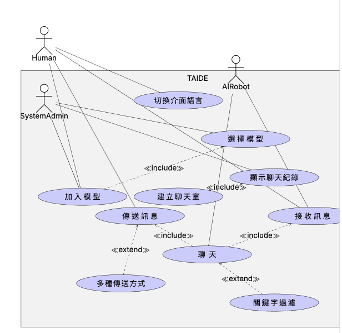
\includegraphics[width=0.45\textwidth]{res/image/usge_casee.png}
    \caption{KUWA+TAIDE 系統使用案例圖}
    \label{fig:use_case}
\end{figure}
\FloatBarrier

\subsection{圖片說明}
此圖 \ref{fig:use_case} 展示了 KUWA 結合 TAIDE 聊天系統的核心功能。圖中定義了三種角色(Actor):
\begin{itemize}
    \item \textbf{Human (使用者)}:主要與系統互動,可進行聊天、選擇模型、傳送與接收訊息。
    \item \textbf{SystemAdmin (系統管理員)}:負責系統層級的操作,如加入新模型、切換介面語言。
    \item \textbf{AIRobot (AI機器人)}:代表後端的 TAIDE 模型,負責處理訊息、生成回應。
\end{itemize}
核心使用案例(Use Case)包括「聊天」、「選擇模型」、「建立聊天室」、「傳送/接收訊息」等,圖中也透過 `<<include>>` 與 `<<extend>>` 關係,說明了各功能之間的依賴與擴充,例如「聊天」功能擴充出「多種傳送方式」與「關鍵字過濾」。此圖清晰地表達了系統的範圍與主要互動情境。

\section{分工結構圖 (Chapter 5)}
分工結構圖(Work Breakdown Structure, WBS)是將專案工作拆解成更小、更易於管理的部分的工具,是專案範疇管理的基礎 \cite{lee2024se}。

\subsection{圖片}
\begin{figure}[htbp]
    \centering
    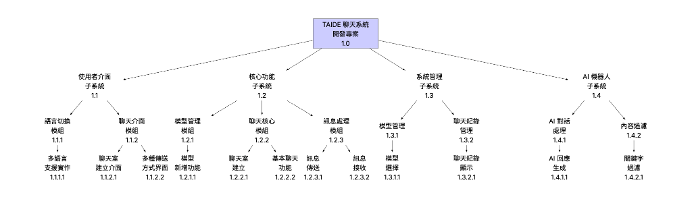
\includegraphics[width=0.45\textwidth]{res/image/wbs.png}
    \caption{KUWA+TAIDE 專案分工結構圖}
    \label{fig:wbs}
\end{figure}
\FloatBarrier

\subsection{圖片說明}
此分工結構圖 \ref{fig:wbs} 以「TAIDE 聊天系統開發專案 (1.0)」為根節點,向下逐層分解。
\begin{itemize}
    \item \textbf{第一層}:將專案分為四個主要子系統:使用者介面 (1.1)、核心功能 (1.2)、系統管理 (1.3) 及 AI 機器人 (1.4)。
    \item \textbf{第二層}:將各子系統進一步細分為具體的模組,例如「使用者介面」分為「語言切換模組」與「聊天介面模組」;「核心功能」則包含「模型管理」、「聊天核心」與「訊息處理」等。
    \item \textbf{第三層之後}:將模組分解為具體的工作包(Work Package),如「聊天介面」下的「聊天室建立介面 (1.1.2.1)」或「訊息處理」下的「訊息傳送 (1.2.3.1)」與「訊息接收 (1.2.3.2)」。
\end{itemize}
此圖有助於清晰地定義專案範疇,並為後續的時程規劃與資源分配提供了基礎。

\section{甘特圖 (Chapter 5)}
甘特圖(Gantt Chart)是一種條狀圖,用以說明專案的時程規劃,顯示各項任務的起始與結束時間 \cite{lee2024se}。

\subsection{圖片}
\begin{figure}[htbp]
    \centering
    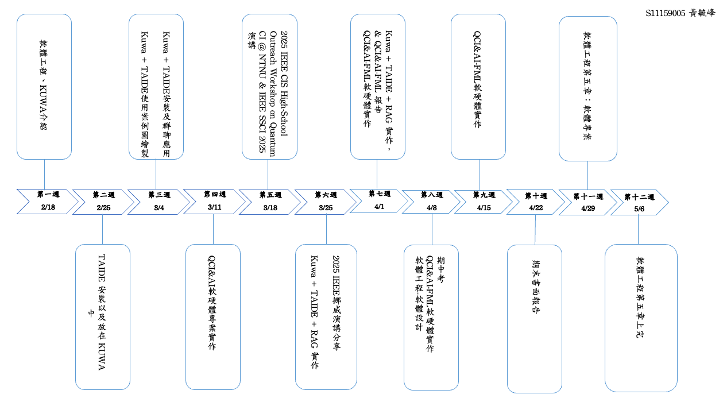
\includegraphics[width=0.48\textwidth]{res/image/時程圖-1.png}
    \caption{專案上半部時程規劃}
    \label{fig:gantt1}
\end{figure}
\begin{figure}[htbp]
    \centering
    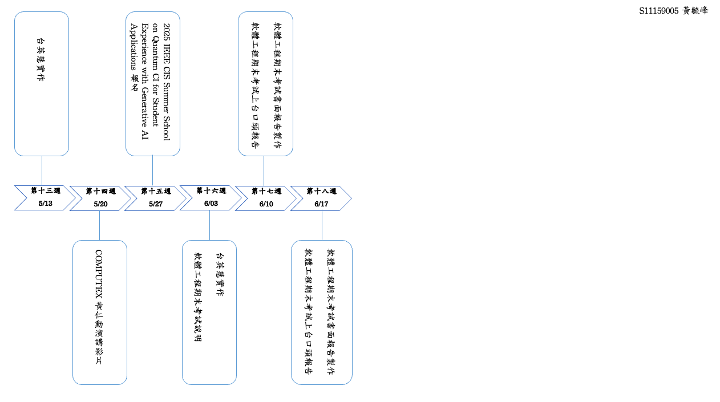
\includegraphics[width=0.48\textwidth]{res/image/時程圖-2.png}
    \caption{專案下半部時程規劃}
    \label{fig:gantt2}
\end{figure}
\FloatBarrier

\subsection{圖片說明}
圖 \ref{fig:gantt1} 與 \ref{fig:gantt2} 共同構成專案的完整甘特圖,展示了從專案啟動到期末報告的各項任務時程。此規劃體現了軟體開發的生命週期,並將模型開發的各階段納入其中:
\begin{itemize}
    \item \textbf{資料模型階段}:對應到時程圖中的「QCI\&AI-FML軟硬體實作」與「資料收集」,此階段專注於定義所需資料的結構、來源與收集方式。
    \item \textbf{知識模型階段}:在「Kuwa + TAIDE + RAG 實作」與「QCI\&AI軟硬體專案實作」中,我們根據收集到的資料建立初步的規則與模型,形成系統的知識基礎。
    \item \textbf{推論模型階段}:此階段的任務是讓模型能夠根據輸入進行推理與回應,體現在「Kuwa + TAIDE使用案例圖繪製」與「台英慧實作」中,我們設計並驗證模型的推論能力。
    \item \textbf{微調模型階段}:在專案後期,如「軟體工程期末考試書面報告製作」階段,我們根據測試結果與新需求,對模型進行持續的微調與優化,以提升其表現。
\end{itemize}
圖中標示的**里程碑 (Milestones)**,如「期中考」、「期末書面報告」等,作為重要的**查核點 (Checkpoints)**,用以檢視專案進度是否符合預期。

\part{QCI軟體平台 \& LLM軟體}

\section{軟體設計 (Chapter 4) :What to do -> How to do}
軟體設計是將使用者需求轉換為具體實作藍圖的過程,回答了「系統要做什麼 (What to do)」以及「如何做到 (How to do)」\cite{lee2024se}。

\subsection{LLM 軟體 (KUWA+TAIDE+RAG)}
\textbf{What to do (功能目標):}
\begin{itemize}
    \item \textbf{實現繁體中文問答能力}:系統需能理解並以流暢的繁體中文進行對話。
    \item \textbf{提供輔助功能}:具備中英翻譯、長文摘要、自動回應等核心功能。
    \item \textbf{支援多樣化部署}:能夠部署於私有(地端)與公有(雲端)環境,滿足不同資安與效能需求。
\end{itemize}
\textbf{How to do (技術實作):}
\begin{itemize}
    \item \textbf{前端與調度 - Kuwa GenAI OS}:使用 Kuwa 作為操作介面,並負責管理與調度後端的 TAIDE 及 RAG 模組。
    \item \textbf{核心模型 - TAIDE}:本地運行 `Llama-3.1-TAIDE-LX-8B` 的量化模型(GGUF 格式),以執行繁體中文的生成、翻譯與摘要任務。
    \item \textbf{知識增強 - RAG 技術}:透過建立向量資料庫,實現檢索增強生成(RAG),讓模型能參考外部知識庫,提供更精準的問答。
\end{itemize}

\subsection{QCI \& AI-FML}
\textbf{What to do (功能目標):}
\begin{itemize}
    \item \textbf{建立 QCI 知識模型}:開發一個用於教育與模擬的 QCI 知識模型。
    \item \textbf{確保隱私與可控性}:強調資料隱私保護,並確保模型運作過程的可監控性。
\end{itemize}
\textbf{How to do (技術實作):}
\begin{itemize}
    \item \textbf{資料收集}:使用 AI-FML 平台的感測器(如攝影機)進行拍照,將影像轉換為文字描述 (Image-to-Text),並將結果儲存於 Excel。
    \item \textbf{知識推理}:建構 QCI 推論模組,透過平台模擬量子狀態與知識推理過程。
    \item \textbf{整合應用}:將 QCI 推論結果與 TAIDE 對話模型整合,打造一個互動式的教學模擬環境。
\end{itemize}

\section{軟體實作細節與成果}
本節將展示 LLM 與 QCI\&AI 兩大專案的具體實作流程與成果。

\subsection{LLM 軟體實作成果}
KUWA+TAIDE+RAG 系統成功在本地環境搭建,實現了具備本地知識庫增強的對話機器人。
\begin{figure}[htbp]
    \centering
    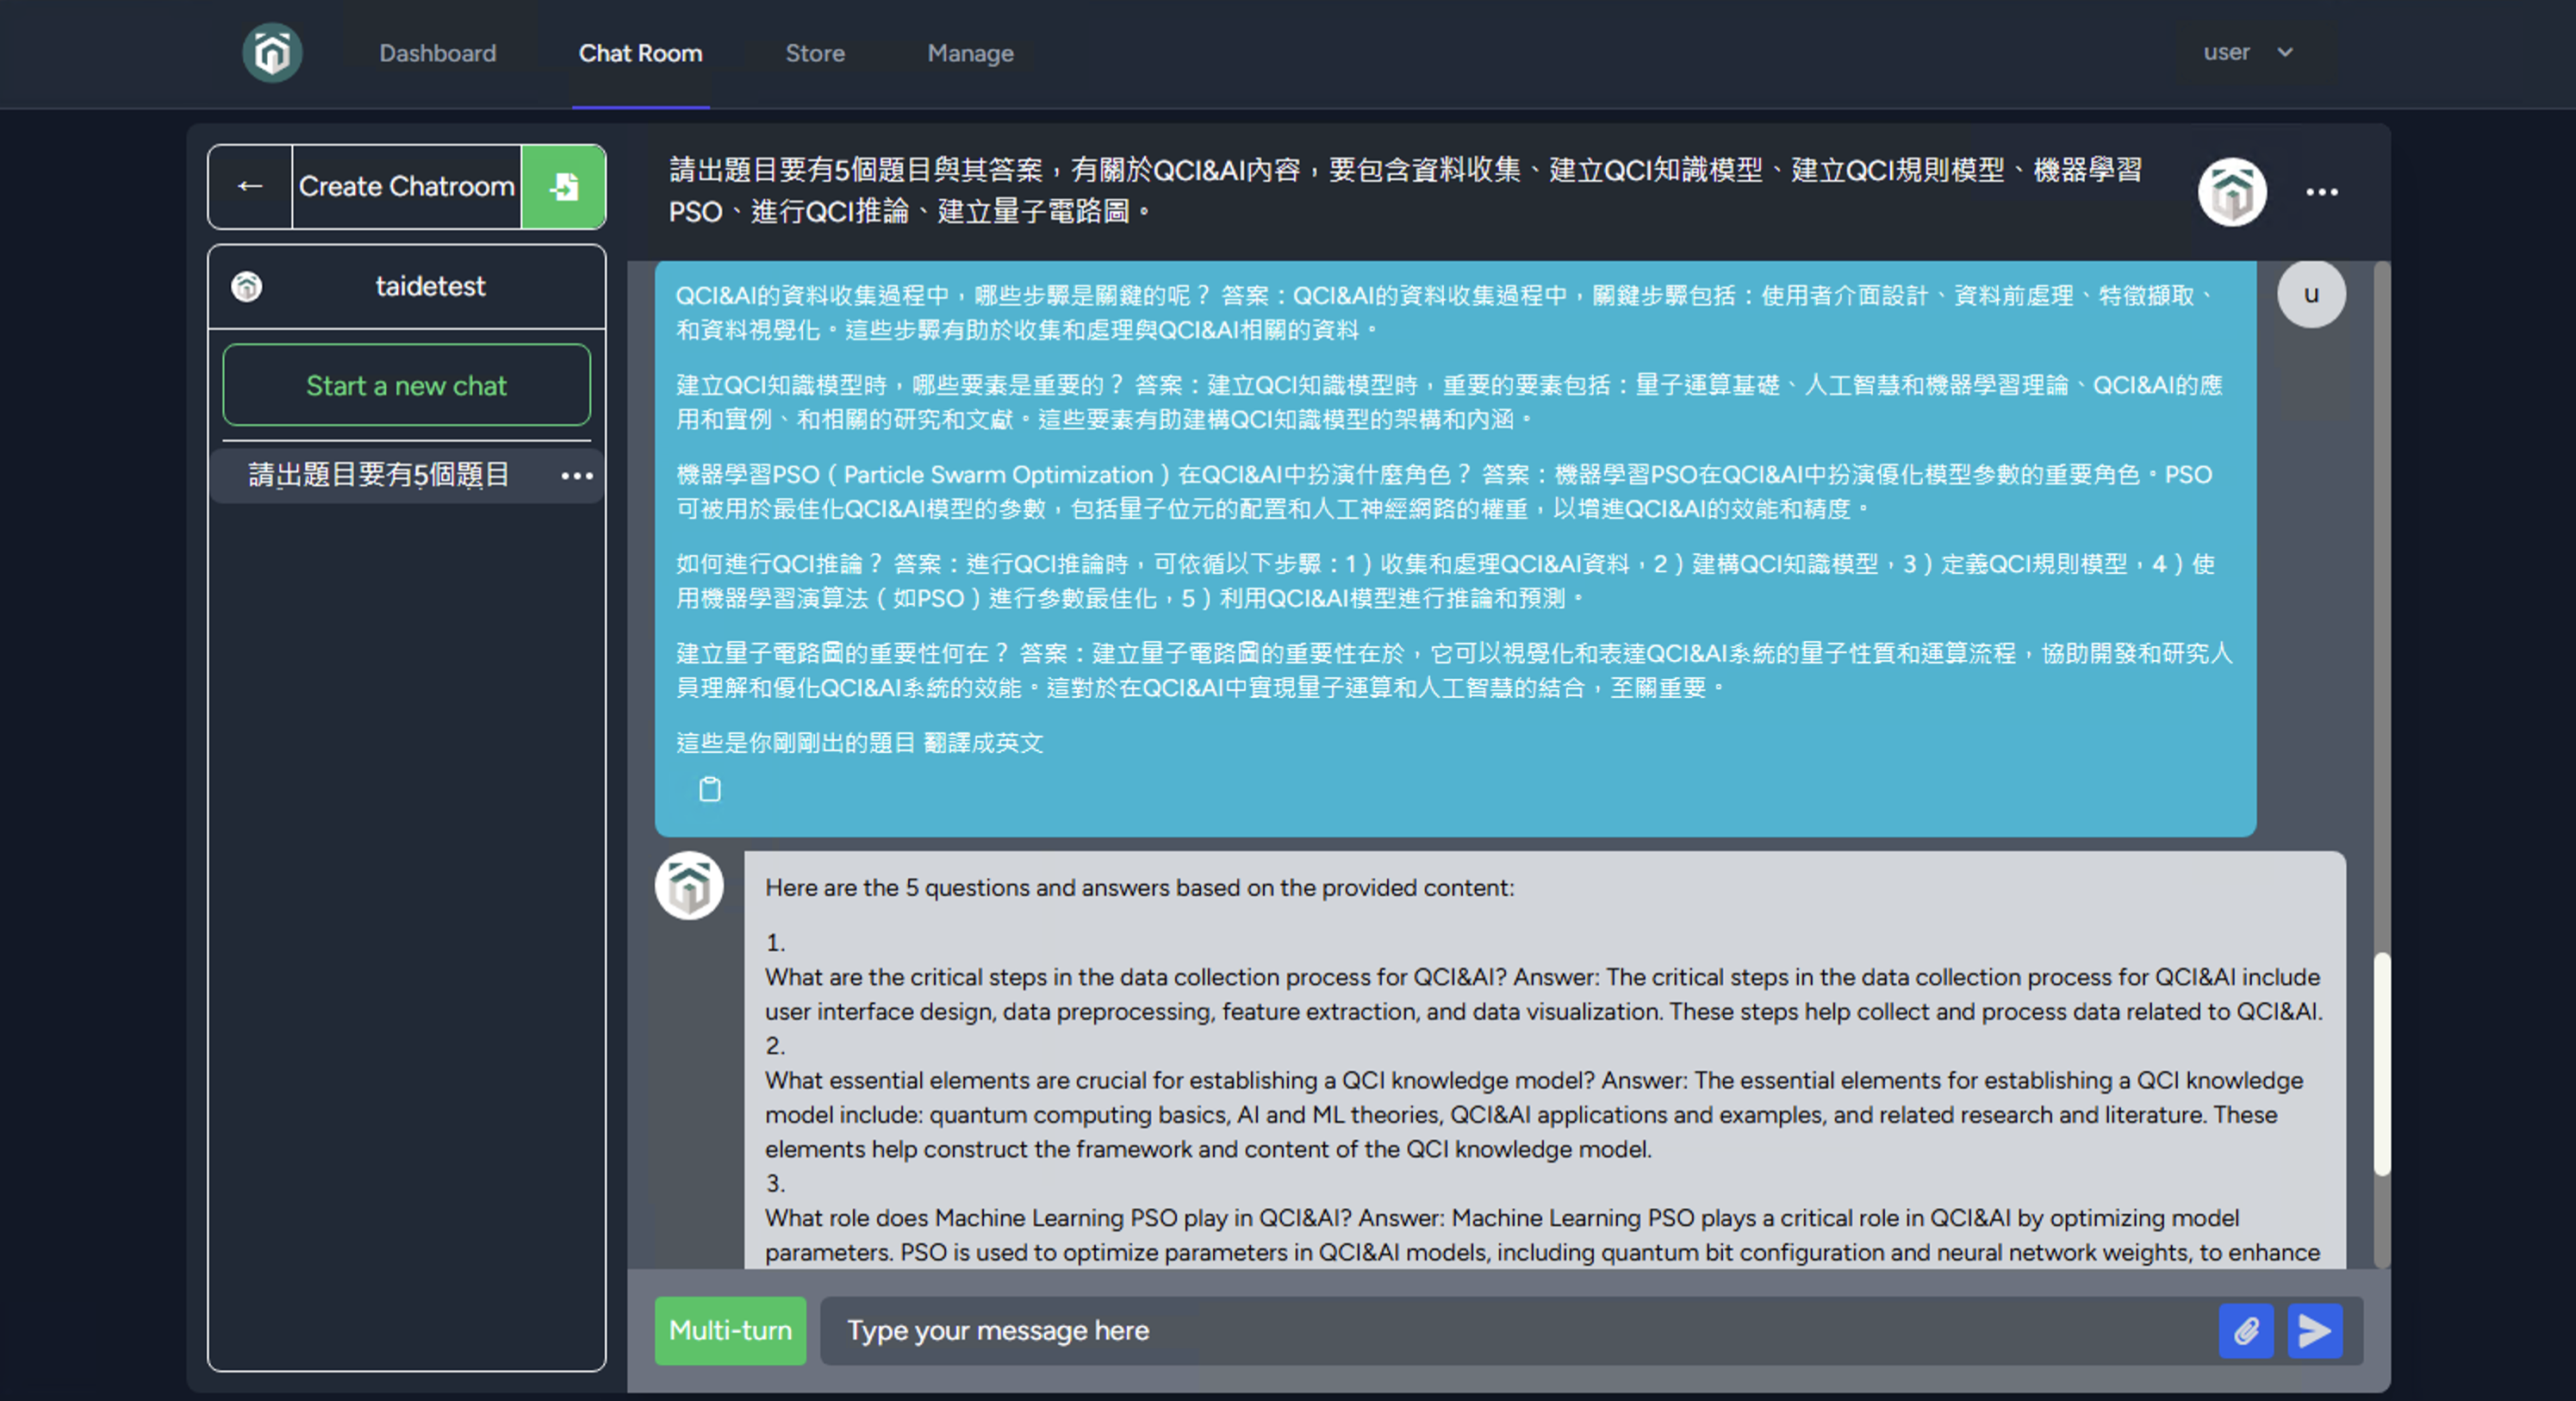
\includegraphics[width=0.48\textwidth]{res/image/taide_chat.png}
    \caption{Kuwa 平台與 TAIDE 模型互動介面}
    \label{fig:taide_chat}
\end{figure}
\begin{figure}[htbp]
    \centering
    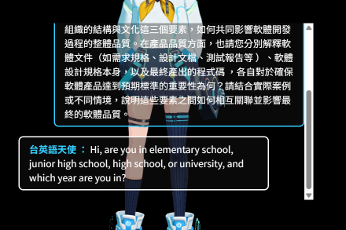
\includegraphics[width=0.48\textwidth]{res/image/台英慧.png}
    \caption{台英慧整合應用,提供多語言學習輔助}
    \label{fig:taiinhei}
\end{figure}
圖 \ref{fig:taide_chat} 展示了使用者透過 Kuwa 平台與本地 TAIDE 模型進行互動的畫面。而圖 \ref{fig:taiinhei} 則為「台英慧」專案的應用實例,此系統整合了 TAIDE 的語言能力,提供台語、英語的共學環境,展現了 LLM 在教育領域的應用潛力。

\subsection{QCI\&AI 實作流程與成果}
QCI\&AI 專案旨在建立一個從資料收集、模型建構到量子推理的完整學習流程。
\begin{enumerate}
    \item \textbf{學習工具與資料收集}:首先,使用圖 \ref{fig:lerning_tool} 所示的 QCI\&AI 學習工具進行資料收集。此工具整合了多種感測器,能夠擷取如圖 \ref{fig:collection_data} 的影像與環境數據。
    \begin{figure}[htbp]
        \centering
        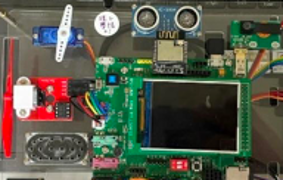
\includegraphics[width=0.48\textwidth]{res/image/lerning_tool.png}
        \caption{QCI\&AI 學習工具硬體}
        \label{fig:lerning_tool}
    \end{figure}
    \begin{figure}[htbp]
        \centering
        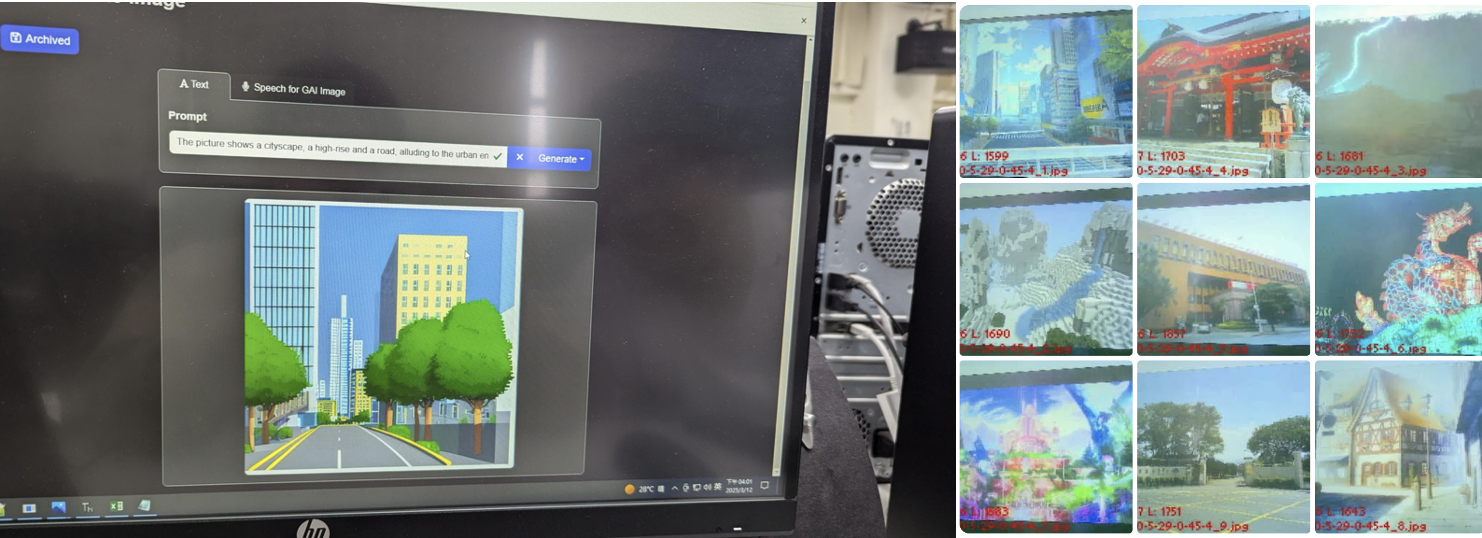
\includegraphics[width=0.48\textwidth]{res/image/collection_data.png}
        \caption{使用學習工具收集的影像資料}
        \label{fig:collection_data}
    \end{figure}
    
    \item \textbf{資料標記與模糊系統實作}:收集到的資料需進行人工標記(如圖 \ref{fig:labeling_train_data}),以建立訓練資料集。接著,我們建構如圖 \ref{fig:model} 所示的模糊推論系統模型,定義輸入(如光線、距離)與輸出之間的模糊關係。
    \begin{figure}[htbp]
        \centering
        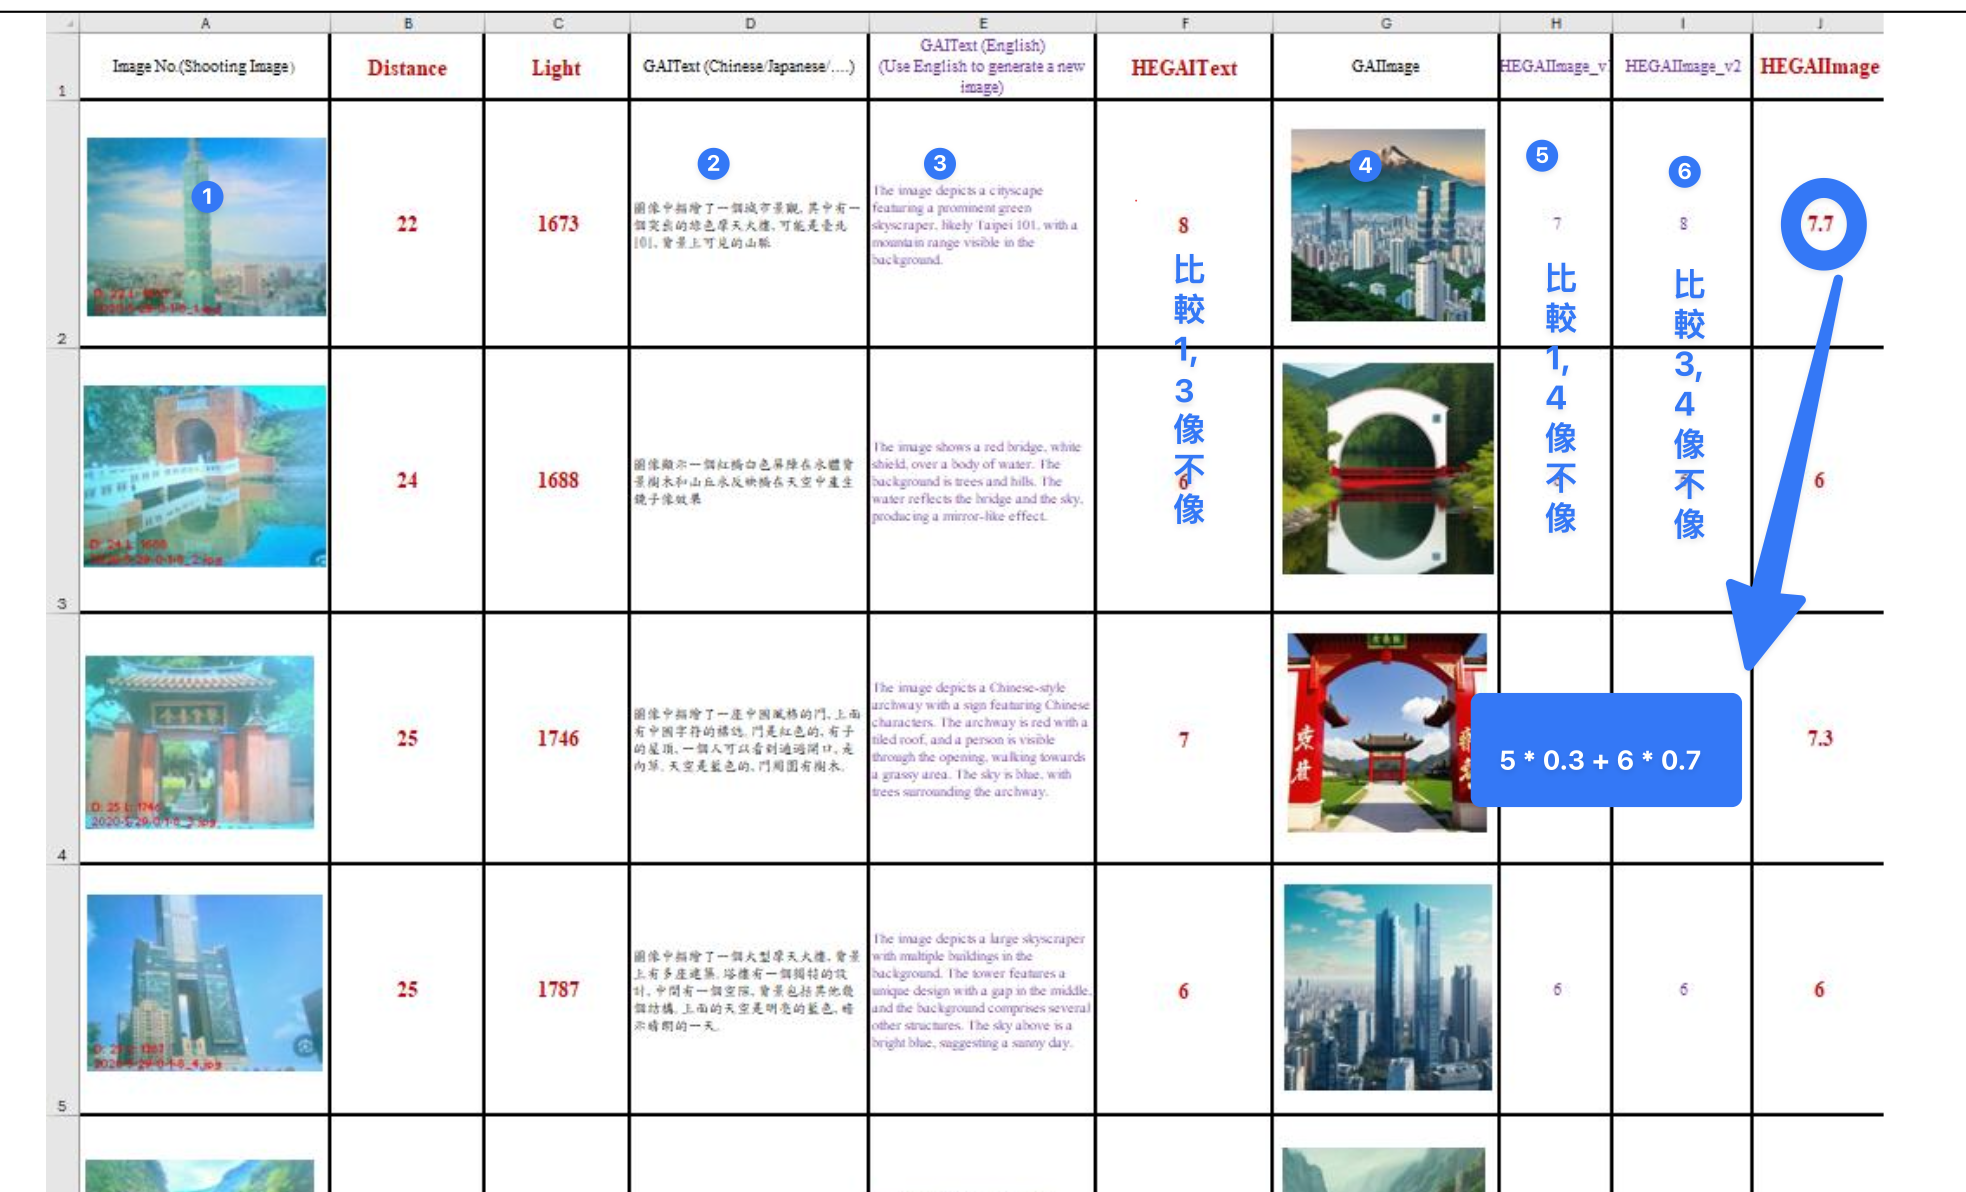
\includegraphics[width=0.48\textwidth]{res/image/labeling_train_data.png}
        \caption{對收集的資料進行標記}
        \label{fig:labeling_train_data}
    \end{figure}
    \begin{figure}[htbp]
        \centering
        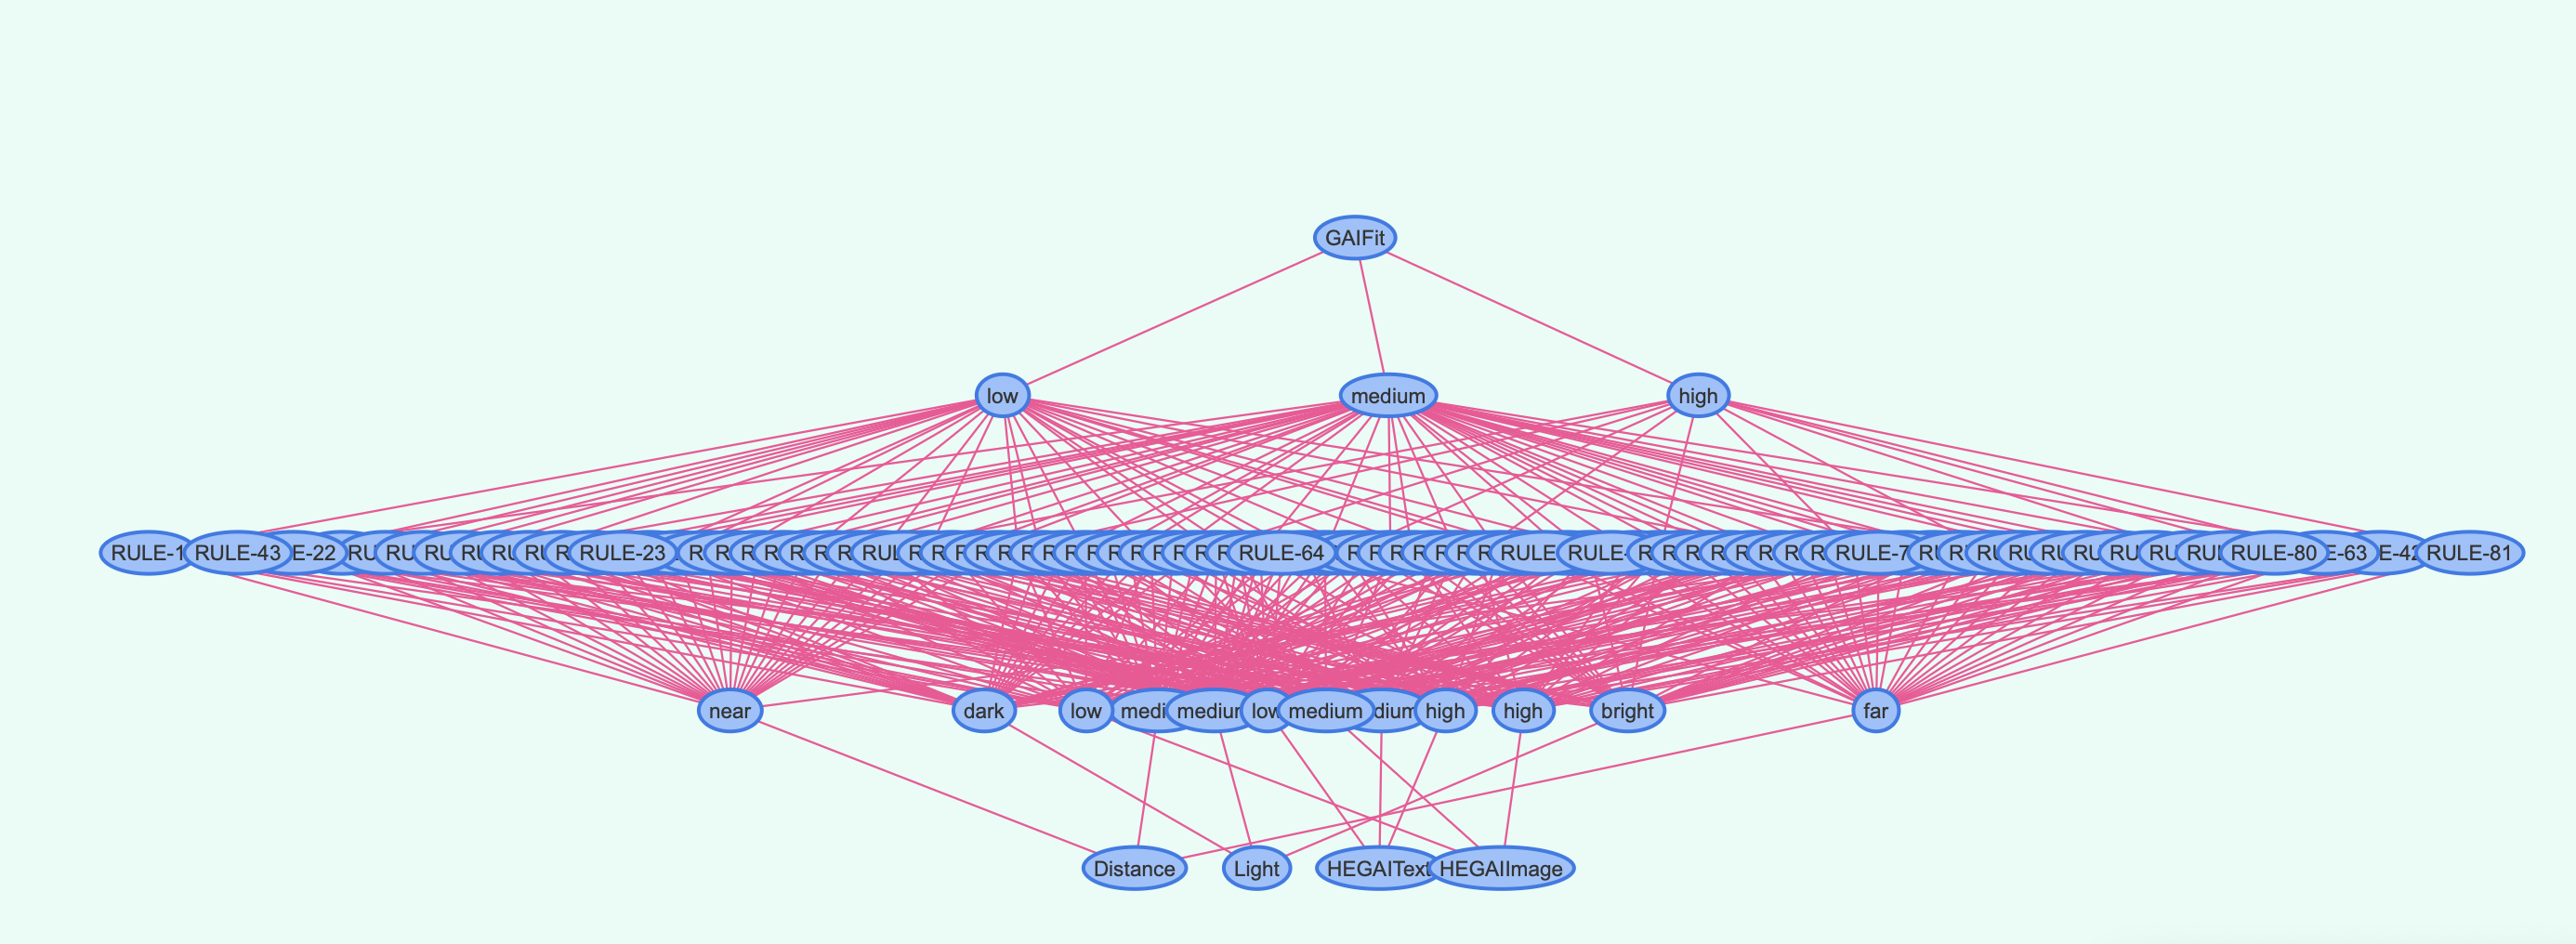
\includegraphics[width=0.48\textwidth]{res/image/model.png}
        \caption{模糊推論系統模型圖}
        \label{fig:model}
    \end{figure}

    \item \textbf{模型訓練與驗證}:透過演化計算對模型進行訓練。圖 \ref{fig:all_BT} 與 \ref{fig:all_AL} 分別展示了知識模型在訓練前後的 T-model 變化,顯示了模型經過學習後的優化情況。
    \begin{figure}[htbp]
        \centering
        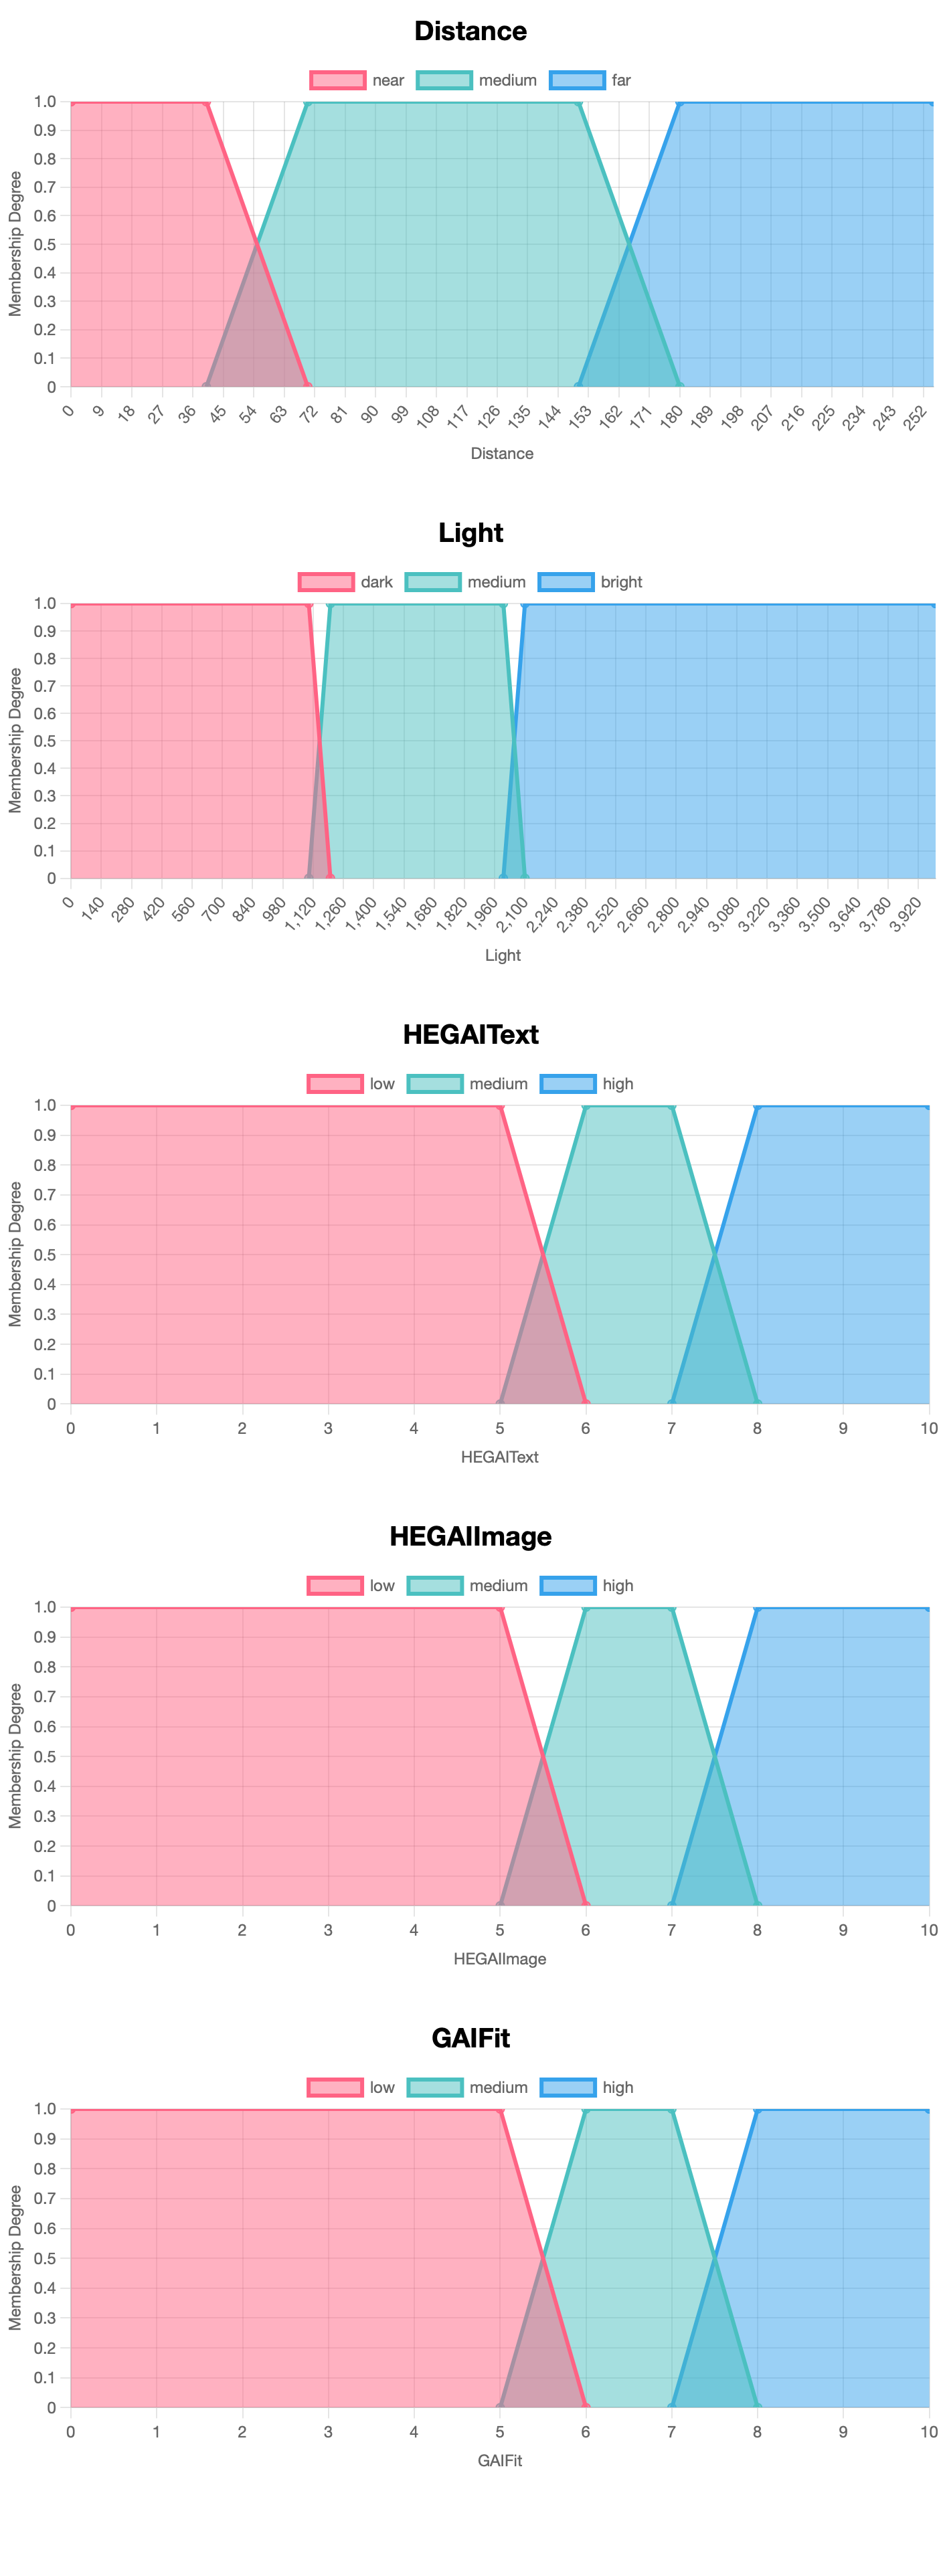
\includegraphics[width=0.48\textwidth]{res/image/all_BT.png}
        \caption{訓練前的 T-model}
        \label{fig:all_BT}
    \end{figure}
    \begin{figure}[htbp]
        \centering
        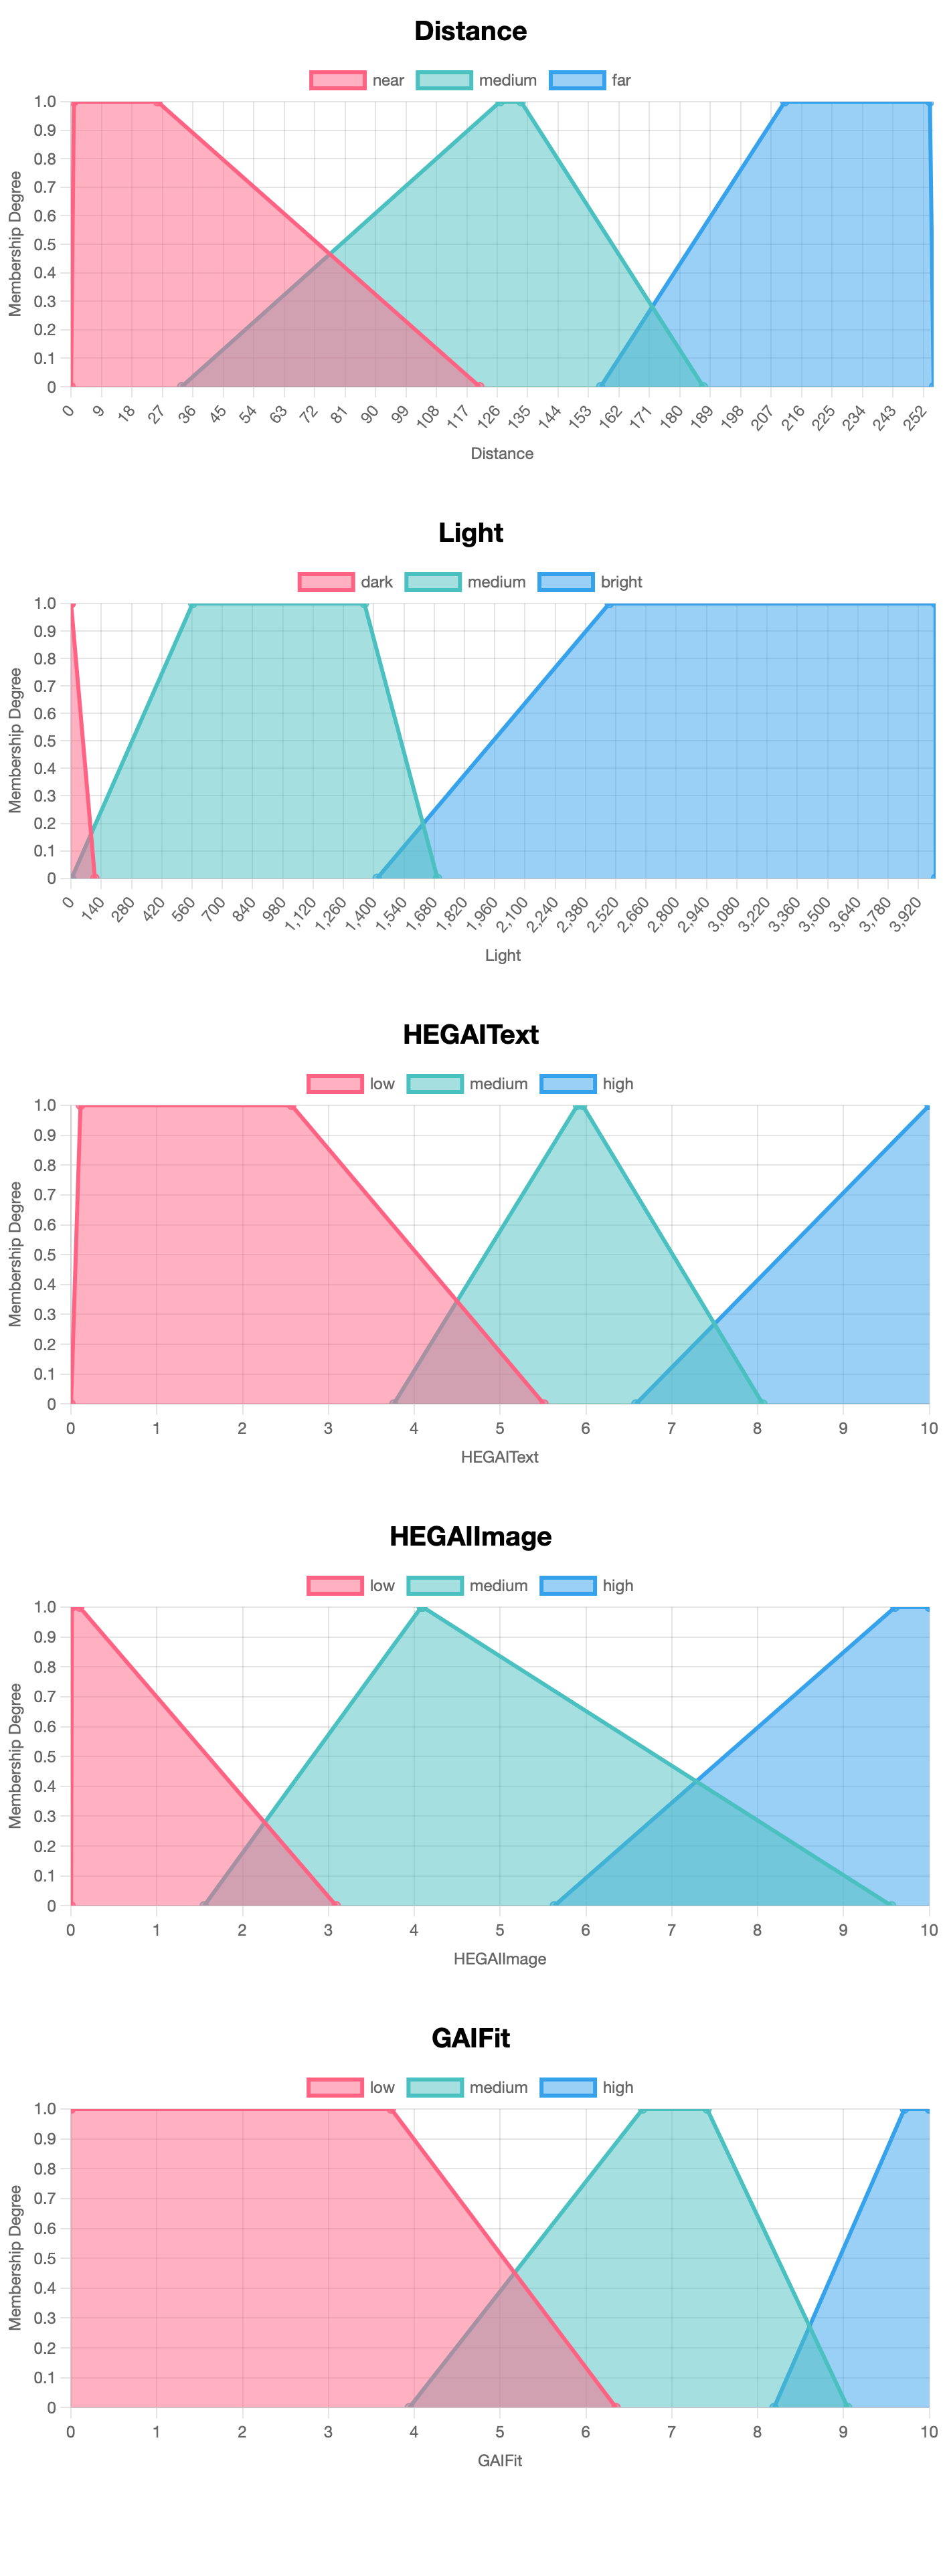
\includegraphics[width=0.48\textwidth]{res/image/all_AL.png}
        \caption{訓練後的 T-model}
        \label{fig:all_AL}
    \end{figure}
    
    \item \textbf{量子模糊推理}:最後,將傳統模糊邏輯模型轉換為量子電路(如圖 \ref{fig:quantum_circuit}),利用量子計算的特性進行推理,探索其在 AI 領域的應用潛力。
    \begin{figure}[htbp]
        \centering
        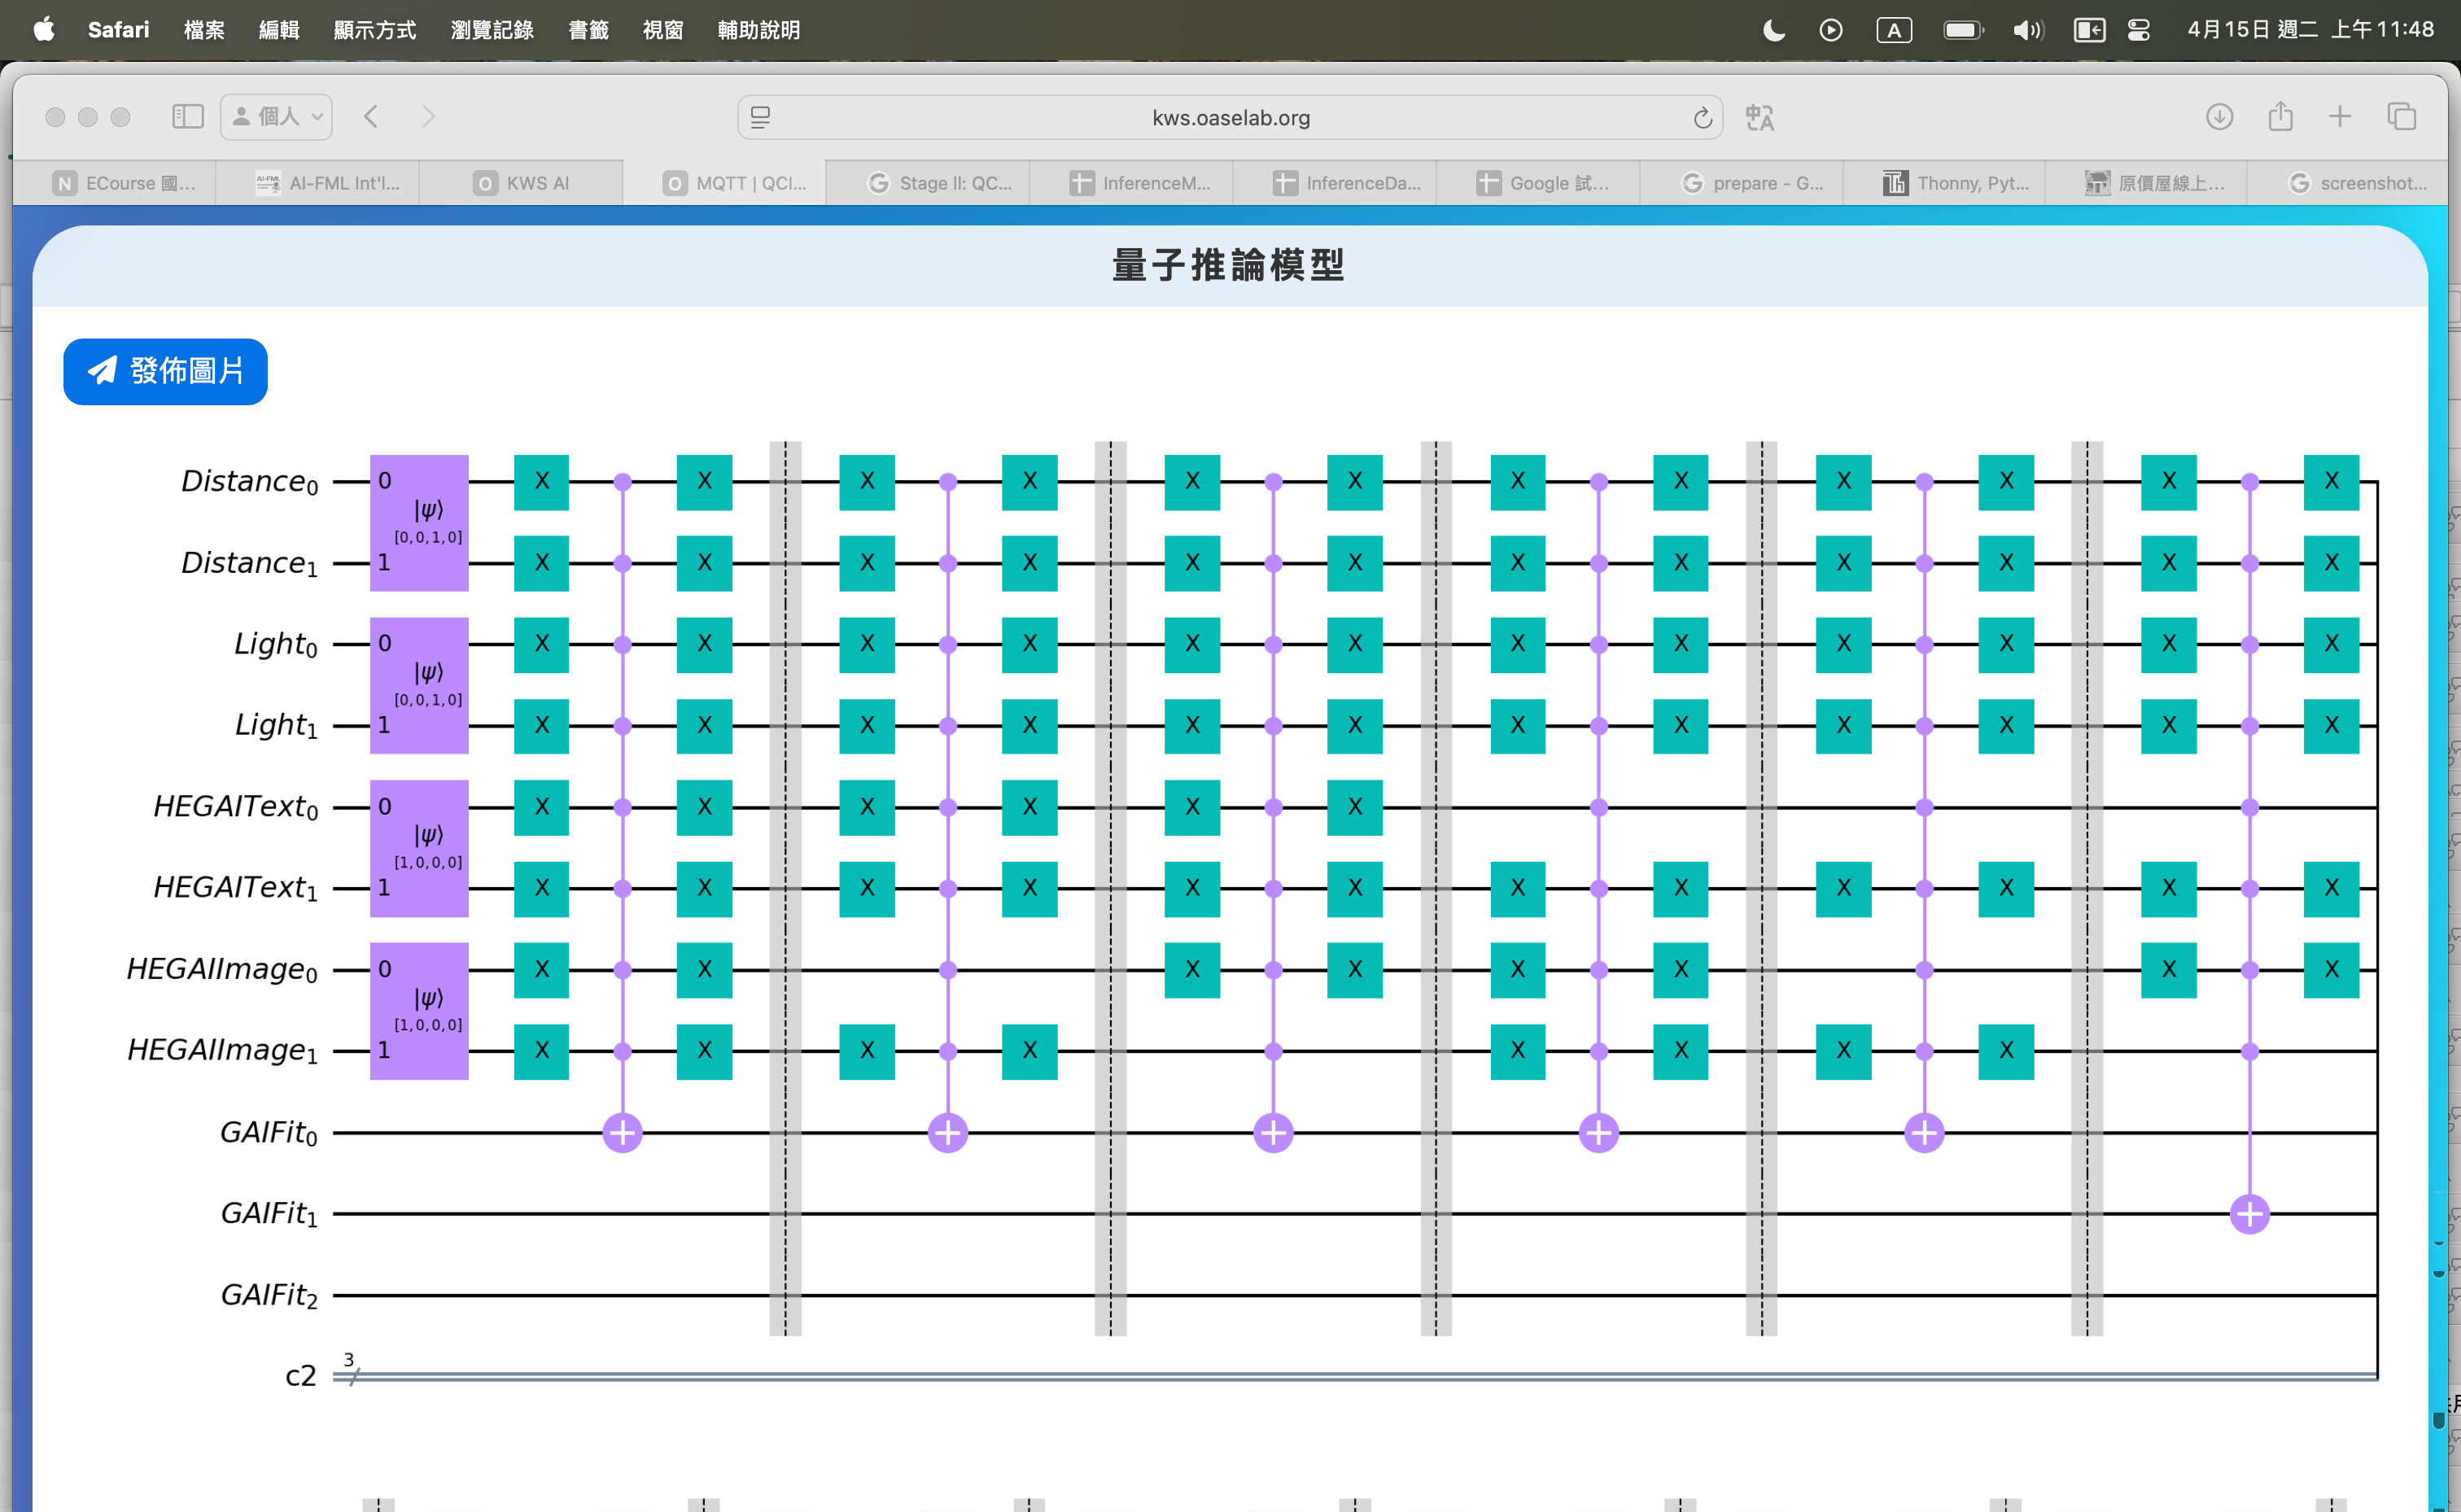
\includegraphics[width=0.48\textwidth]{res/image/quantum.png}
        \caption{量子模糊推理的量子電路實現}
        \label{fig:quantum_circuit}
    \end{figure}
\end{enumerate}


\section{軟體測試 (Chapter 6)}
軟體測試是驗證與確認軟體是否滿足其設計要求及使用者期望的關鍵過程 \cite{lee2024se}。本專案主要採用黑箱測試 (Black-box Testing) 的方法。

\subsection{LLM 軟體測試}
\textbf{測試目標:}
\begin{itemize}
    \item 驗證系統能正確理解繁體中文問題。
    \item 確保回應內容符合教學、翻譯、摘要等特定需求。
    \item 在不同輸入下,系統能保持回應的穩定性與品質。
\end{itemize}
\textbf{測試方法與策略 (動態測試):}
\begin{enumerate}
    \item \textbf{單元測試 (Unit Testing)}:針對單一功能進行測試,如輸入一則英文新聞,驗證 TAIDE 模型的摘要功能是否能產出合理的中文摘要。
    \item \textbf{整合測試 (Integration Testing)}:測試模組間的協作,例如,上傳一份文件至 RAG 知識庫後,向 TAIDE 提問與文件相關的問題,驗證 RAG 是否成功擷取資訊並由 TAIDE 正確生成答案。
    \item \textbf{系統測試 (System Testing)}:對整個系統進行端到端的測試,模擬使用者從開啟 Kuwa、選擇 TAIDE+RAG 模型到完成一次完整問答的流程,確保整體運作流暢。
\end{enumerate}

\subsection{QCI \& AI-FML 測試}
\textbf{測試目標:}
\begin{itemize}
    \item 確保 AI-FML 平台能成功完成感測器資料的上傳、轉換與儲存。
    \item 驗證 QCI 推論模組能否根據輸入生成合乎邏輯的知識回應。
\end{itemize}
\textbf{測試方法與策略 (動態測試):}
\begin{enumerate}
    \item 拍攝一張包含特定物件的環境圖片。
    \item 透過 Image-to-Text 功能將其轉換為文字描述。
    \item 將文字描述輸入至 QCI 推論模組。
    \item 觀察與分析輸出回應是否符合實際情境與預期邏輯。
\end{enumerate}

\subsection{測試結果分析}
在模型訓練與微調過程中,我們記錄了準確率 (Accuracy)、均方誤差 (Mean Squared Error, MSE) 與均方根誤差 (Root Mean Squared Error, RMSE) 等指標,以進行動態評估。
\begin{figure}[htbp]
    \centering
    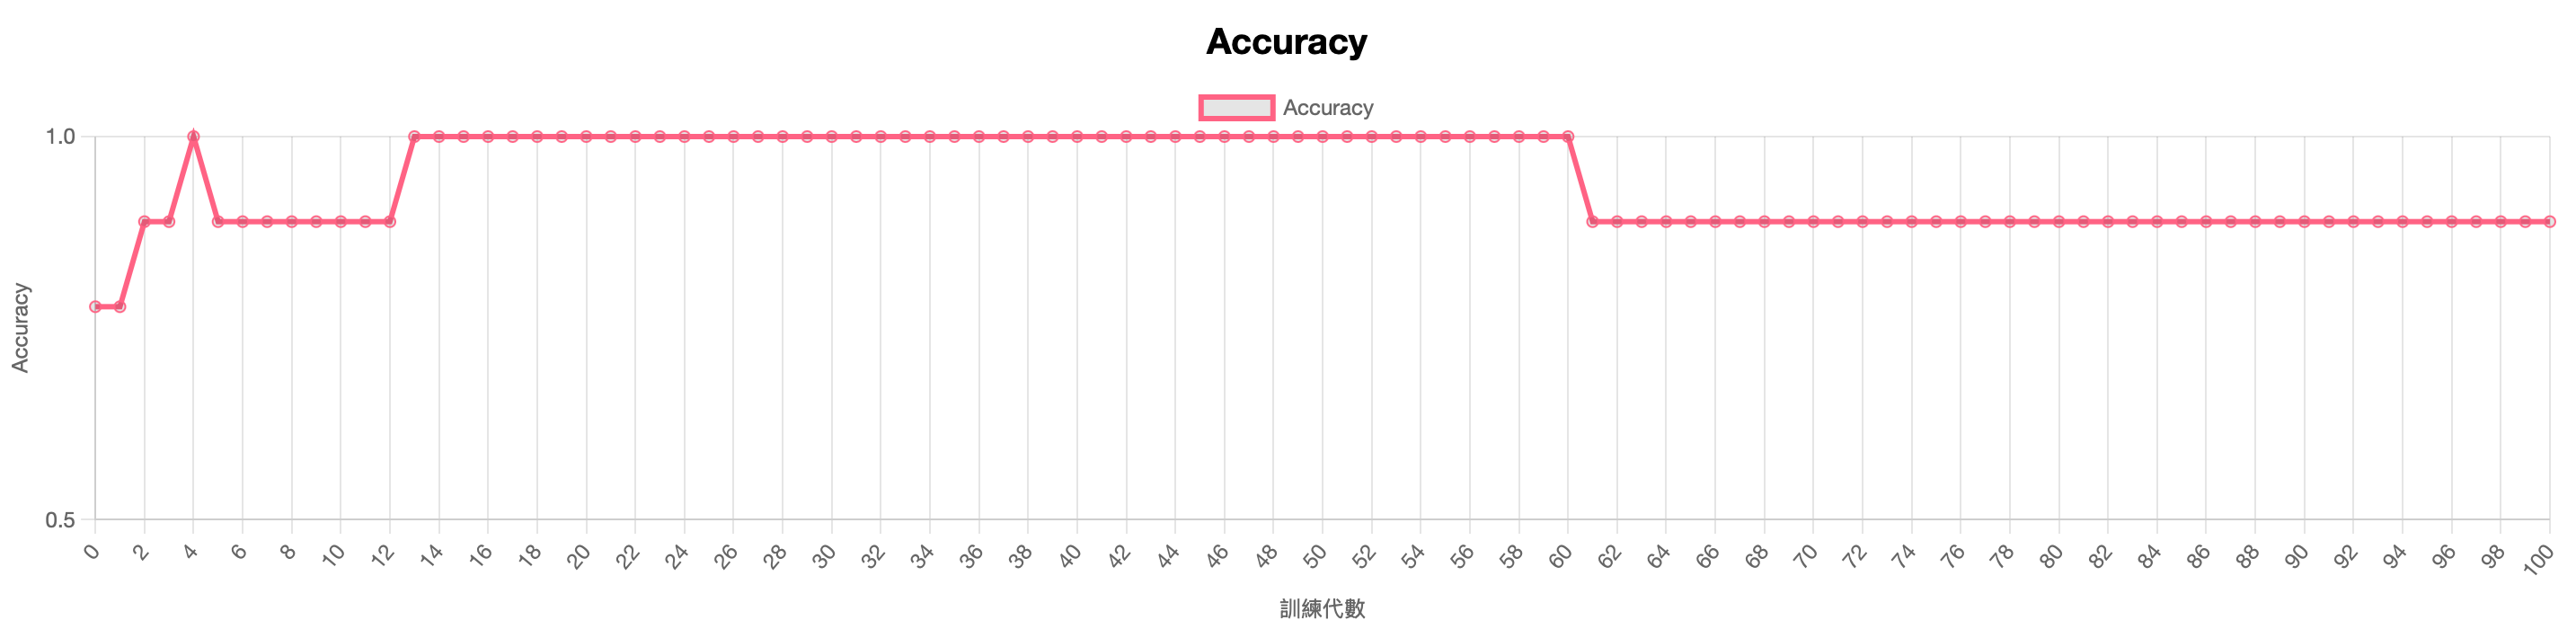
\includegraphics[width=0.45\textwidth]{res/image/accuracy.png}
    \caption{模型準確率曲線}
    \label{fig:accuracy_curve}
\end{figure}
\begin{figure}[htbp]
    \centering
    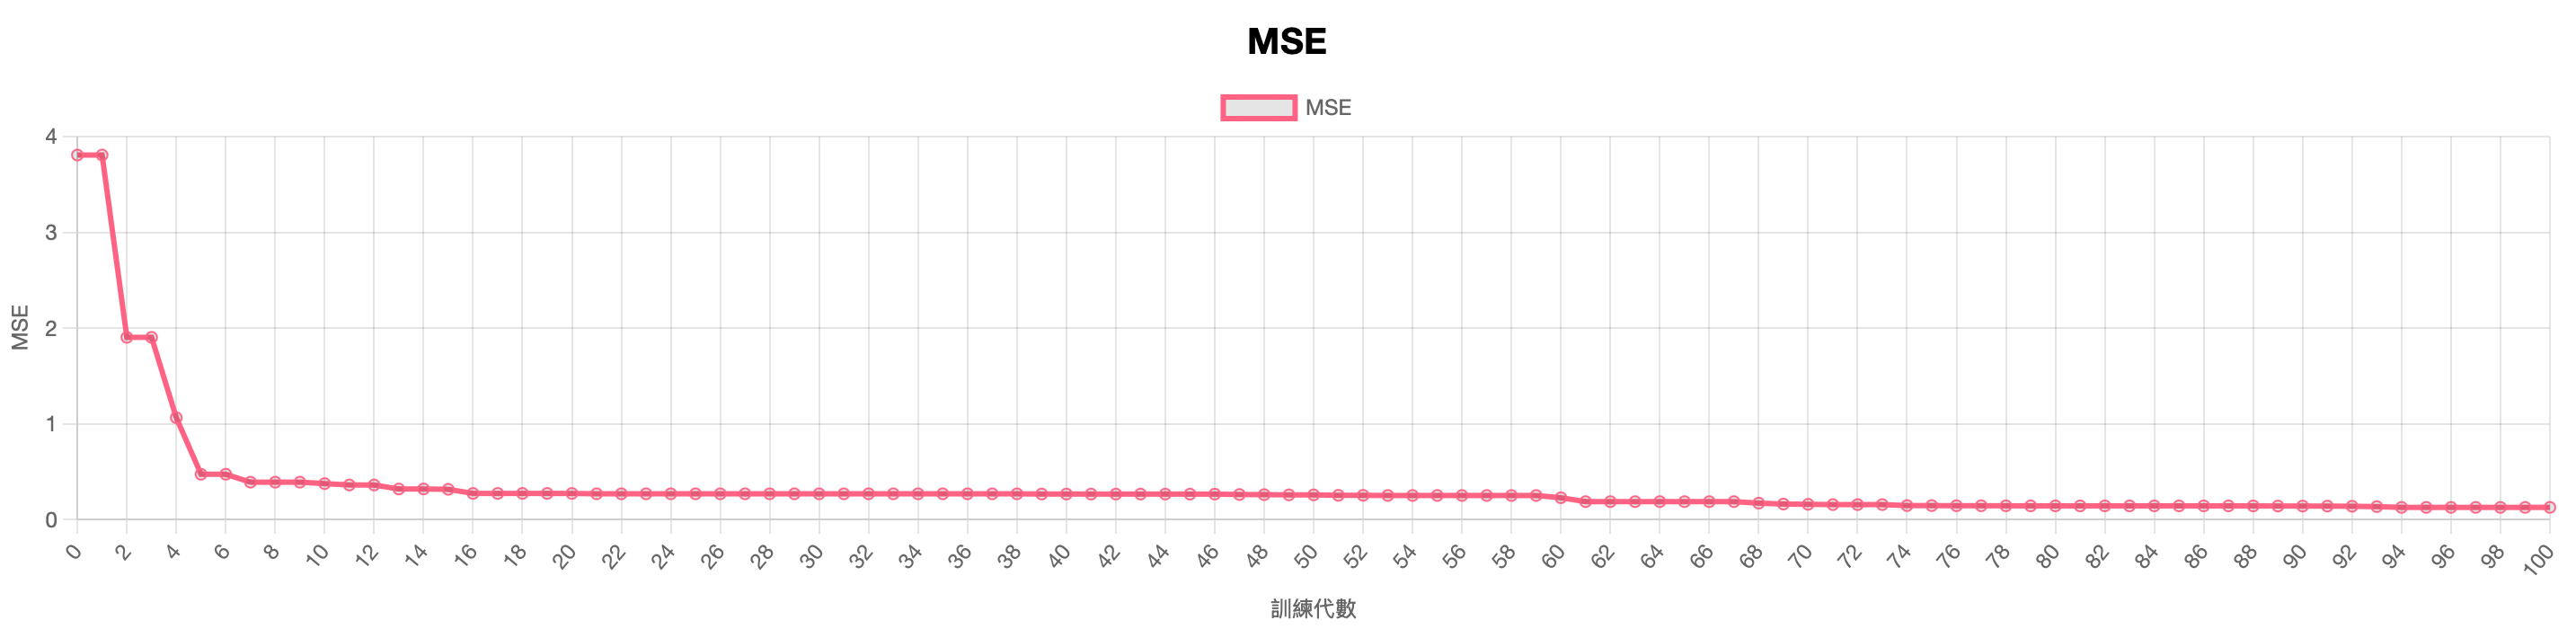
\includegraphics[width=0.45\textwidth]{res/image/mse.png}
    \caption{模型均方誤差曲線}
    \label{fig:mse_curve}
\end{figure}
\begin{figure}[htbp]
    \centering
    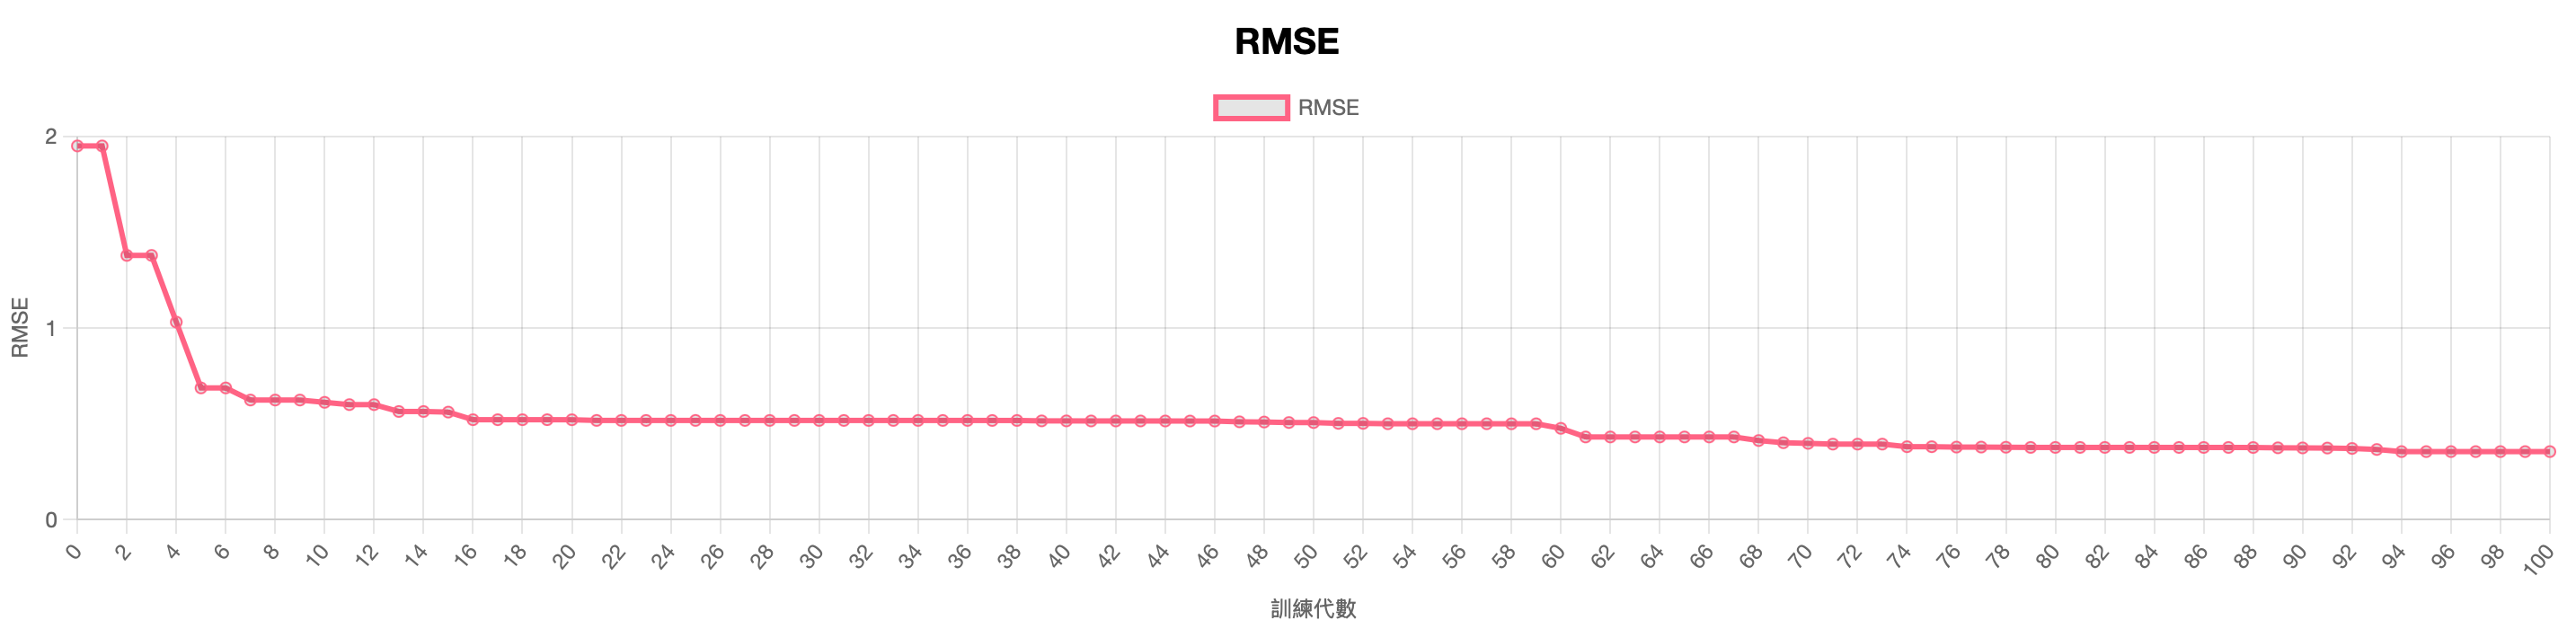
\includegraphics[width=0.45\textwidth]{res/image/rmse.png}
    \caption{模型均方根誤差曲線}
    \label{fig:rmse_curve}
\end{figure}

如圖 \ref{fig:accuracy_curve} 所示,模型的準確率隨著訓練代數增加而穩定提升並收斂。同時,圖 \ref{fig:mse_curve} 和 \ref{fig:rmse_curve} 中的 MSE 與 RMSE 值則穩定下降,顯示模型的預測誤差持續減小。這些數據共同驗證了我們的訓練與測試策略是有效的,模型品質得到了持續改善。

\section{軟體品質保證與管理 (Chapter 7, 8, 9)}
為了確保最終產出的品質,除了測試之外,更需要全面性的品質保證、建構管理與正規方法論的思維。

\subsection{軟體品質保證 (Chapter 7)}
軟體品質保證(Software Quality Assurance, SQA)是確保軟體開發流程與產出符合預定標準的一系列活動 \cite{lee2024se}。
\textbf{LLM 軟體品質保證:}
\begin{itemize}
    \item \textbf{客戶需求}:繁體中文準確回應 $\rightarrow$ \textbf{品質特性}:使用本地部署的 TAIDE 模型(繁中特化微調)。
    \item \textbf{客戶需求}:低延遲、即時反應 $\rightarrow$ \textbf{品質特性}:啟用量化模型 (Q4\_K\_M) 與 RAG 快取機制。
\end{itemize}
\textbf{QCI \& AI-FML 品質保證:}
\begin{itemize}
    \item \textbf{客戶需求}:可從照片或語音取得知識 $\rightarrow$ \textbf{品質特性}:建置 Image-to-Text/Voice 轉換模組。
    \item \textbf{客戶需求}:推論邏輯要解釋清楚 $\rightarrow$ \textbf{品質特性}:QCI 模組以量子態圖形/表格輸出解釋結果。
\end{itemize}

\subsection{軟體建構管理 (Chapter 8)}
軟體建構管理(Software Configuration Management, SCM)旨在於整個軟體生命週期中,有系統地管理與控制軟體產品的變更 \cite{lee2024se}。在本專案中,SCM體現於:
\begin{itemize}
    \item \textbf{建構識別 (Identification)}:明確定義所有納管的建構項目(Configuration Item, CI),例如 TAIDE 模型的不同量化版本、RAG 的知識庫文件、系統的原始碼與需求規格書。
    \item \textbf{版本控制 (Control)}:我們使用 Git 作為版本控制工具,所有程式碼的修改都透過 commit 進行記錄,重要的版本發布(如完成某項功能)則透過 tag 進行標記,實現了變更的追溯與管理。
    \item \textbf{狀態報告 (Status Accounting)}:Git 的提交歷史(log)即為一種狀態報告,記錄了每一次變更的作者、時間與內容,讓團隊成員了解專案的演進狀態。
    \item \textbf{建構稽核 (Auditing)}:在整合新功能前,透過 Code Review 來稽核程式碼是否符合規範,確保變更的品質,這是一種非正式的建構稽核。
\end{itemize}

\subsection{正規方法論之應用 (Chapter 9)}
正規方法論(Formal Methods)是使用具備嚴謹數學基礎的語言來描述與驗證系統,能大幅減少規格的模糊性,提升軟體可靠度 \cite{lee2024se}。雖然本專案未完全採用正規方法論開發,但其概念對提升品質有重要啟發:
\begin{itemize}
    \item \textbf{概念應用}:在定義 LLM 功能時,我們可以借鑒正規方法論的思維,力求規格的精確。例如,與其模糊地描述「系統應能摘要文章」,不如定義「給定一篇長度不超過N個字元的文章,系統應產出一篇長度為原文10\%$\pm$2\%且包含原文核心論點的摘要」。
    \item \textbf{未來展望}:對於系統中如 RAG 檢索邏輯等核心部分,未來可考慮使用物件限制語言 (Object Constraint Language, OCL) 來為對應的UML模型(如類別圖)添加限制條件,以數學方式確保「檢索出的文件必須與使用者提問的關鍵字相關度高於門檻值 T」,從而形式化地保證系統的正確性。
\end{itemize}


\part{生成式AI工具對我學習軟體工程之分析}

\section{生成式AI工具對我學習軟體工程分析}

\subsection{正面效益}
生成式AI工具對我的學習帶來了顯著的正面效益。
\begin{itemize}
    \item \textbf{範例:快速理解抽象概念}:當學習軟體設計模式 (Design Patterns) 時,像「抽象工廠模式 (Abstract Factory Pattern)」這樣的概念僅閱讀文字定義很難完全理解。我會要求 TAIDE 提供一個具體的 Java 或 Python 程式碼範例,例如「請用抽象工廠模式寫一個能建立不同品牌(如 Dell 和 Apple)電腦元件(CPU、RAM)的程式碼」。透過實際可運行的程式碼,我可以更快地掌握其結構與應用場景。
    \item \textbf{範例:輔助除錯 (Debugging)}:在開發過程中,我遇到一段 Python 程式碼在處理檔案路徑時,在 Windows 上正常,但在 Linux 環境下出錯。我將相關程式碼片段貼給 AI,並詢問「這段程式碼為何在 Linux 會出錯?」。AI迅速指出 Windows 的路徑分隔符 `\` 與 Linux 的 `/` 不同,並建議使用 `os.path.join()` 來確保跨平台相容性。這為我節省了大量的搜尋和嘗試時間。
\end{itemize}

\subsection{負面影響}
然而,過度依賴生成式AI也帶來了一些負面影響。
\begin{itemize}
    \item \textbf{範例:產生錯誤資訊(幻覺)}:有一次我詢問一個較為冷門的函式庫的特定用法,AI 提供了一段看起來非常合理的程式碼,但我實際執行時卻頻頻報錯,提示某個函式不存在。經過查證官方文件,我才發現 AI 杜撰(產生幻覺)了一個不存在的函式。這個經驗讓我明白,對於 AI 提供的資訊,尤其是非主流的技術知識,必須抱持懷疑態度並親自驗證。
    \item \textbf{範例:削弱獨立解決問題的能力}:在專案初期,我習慣於一遇到問題就立刻詢問 AI,而不是先自己思考或查閱資料。這導致我對基礎知識的掌握不夠牢固。後來我調整了學習策略,強迫自己先嘗試獨立解決問題至少15分鐘,若仍無頭緒才向 AI 求助。這幫助我重新建立了獨立思考和解決問題的習慣。
\end{itemize}

\subsection{整體效益}
對我而言,使用生成式AI工具學習軟體工程的**整體效益是正面的**。儘管存在產生錯誤資訊和可能導致依賴的風險,但只要能建立起「驗證」和「自律」的習慣,AI 就是一個極其強大的學習加速器。它能將我從繁瑣的資訊搜尋和基礎程式碼撰寫中解放出來,讓我能更專注於理解核心的架構設計與演算法思想。總體來說,它是一個非常有用的工具,是助力而非阻力。

\subsection{課程學習心得}
這門軟體工程課程讓我收穫良多。感謝李健興老師的悉心指導,以及課本作者李允中老師提供的紮實理論基礎。透過課程,我不僅系統性地學習了軟體開發的生命週期、需求工程、設計與測試等核心知識,更重要的是,課程結合了 QCI\&AI 與 LLM 等前沿技術的實作,讓我能親手將理論應用於實踐。從安裝設定 Kuwa 平台,到訓練與驗證模型,每一步都加深了我對軟體工程的理解。感謝助教們的耐心協助,讓我在遇到困難時能及時獲得解決。這門課讓我對軟體工程有了全新的認知,是一次理論與實務完美結合的寶貴學習經驗。

\section*{致謝}
本報告的完成,誠摯感謝指導教授李健興博士在
Software Engineering 與 QCI\&AI 領域的專業指導和啟發。
同時,特別感謝國立臺南大學與國立高雄大學以及國家高速網路計算中心提供的學術資源與支持環境。
對於 KuwaAI 團隊提供的 KUWA 及 TAIDE 團隊提供的 LLaMA-TAIDE 3.1 8B 模型以及好心人提供的 LLaMA-TAIDE 3.1 8B Q4 KM 量化模型,
使得本報告的實作部分得以順利進行,在此表達由衷謝意。
最後,感謝所有提供建議的同學們以及幫助我的助教們,沒有他們我無法完成這份報告。

% References
\begin{thebibliography}{9}

\bibitem{lee2025outreach}
C.-S. Lee, M.-H. Wang, and Y.-J. Lin. “2025 IEEE CIS High-School Outreach Activity Report Workshop on Quantum CI @ NTNU \& IEEE SSCI 2025: A Sandbox for Teaching and Learning in Quantum CI for Pre-University and Undergraduate Students.” National University of Tainan. Accessed: May 19, 2025. [Online]. Available: Internal document (no public link).

\bibitem{lee2025fuzzy}
C.-H. Lee. “LLM-based Fuzzy Agent for Human-Machine Interaction in STEM Education and Taiwanese-English Co-Learning Application.” National University of Tainan @ The Hong Kong Polytechnic University. Accessed: May 19, 2025. [Online]. Available: Conference presentation (no public link).

\bibitem{lee2024se}
Y.-C. Lee. “軟體工程 Software Engineering.” National Taiwan University. Published: Oct. 11, 2024. Accessed: May 19, 2025. [Online]. Available: Internal course material.

\bibitem{kws_ai_team}
KWS AI Team. “NUTN-TAIDE-TW Chat.” KWS AI Platform. Accessed: May 19, 2025. [Online]. Available: https://kws.oaselab.org/llama-chat/

\bibitem{qciai_fml_team}
QCI\&AI-FML Team. “QCI\&AI-FML 學習平台.” QCI\&AI Learning Platform. Accessed: May 19, 2025. [Online]. Available: https://kws.oaselab.org/qciai/

\bibitem{aifml_academy}
AI-FML Academy. “AI-FML 國際學院.” AI-FML International Academy. Accessed: May 19, 2025. [Online]. Available: https://sites.google.com/asap.nutn.edu.tw/ai-fml-international-academy/home

\bibitem{taide_project}
TAIDE Project. “TAIDE - 推動臺灣可信任生成式 AI 發展計畫.” TAIDE. Accessed: May 19, 2025. [Online]. Available: https://taide.tw/index

\bibitem{taide_huggingface}
TAIDE Team. “TAIDE Hugging Face.” Hugging Face. Accessed: May 19, 2025. [Online]. Available: https://huggingface.co/taide

\bibitem{kuwa_github}
KuwaAI, *GenAI OS*. [Online]. Available: \url{https://github.com/kuwaai/genai-os}. Accessed: June 14, 2025.


\end{thebibliography}


\end{document}
